
\section{Auswertung}
Die Mittelwerte und Fehler der errechneten Größen in den folgenden Abschnitten lassen
sich mit folgenden Formeln bestimmen und werden an die jeweiligen Toleranzen angepasst:
\begin{equation}
  \bar{x} = \frac{1}{n} \sum{x_n}
  \label{eqn:Mittelwert}
\end{equation}

\begin{equation}
\upsigma = \frac{1}{\sqrt{n}} \sqrt{\frac{\sum{(x_n - \bar{x})^2}}{n-1} }
\label{eqn:Standardabweichung}
\end{equation}

\subsection{Wheatstonesche Brückenschaltung}
\begin{table}
  \centering
  \caption{Gemessene Werte bei der Wheatstoneschen Brücke}
  \label{tab:Wheatstone}
  \begin{tabular}{ c c c c c }
    \toprule
      & & Messung 1 & Messung 2 & Messung 3 \\
    \midrule
    Wert 10 & \multicolumn{1}{c|}{$\su{R_2}$  in  $\su{\Omega} $ } & 500 & 664 & 1000 \\
            & \multicolumn{1}{c|}{$\su{R_3}$  in  $\su{\Omega} $ } & 321 & 261 & 198  \\
            & \multicolumn{1}{c|}{$\su{R_4}$  in  $\su{\Omega} $ } & 679 & 739 & 802 \\
            & \multicolumn{1}{c|}{$\su{R_x}$  in  $\su{\Omega} $ } & 236.38 & 234.51 & 246.88  \\
            & \multicolumn{1}{c|}{$\su{\Delta R_x}$  in  $\su{\Omega} $ } & \pm 1.27 & \pm 1.26 & \pm 1.33  \\
    \midrule
    Wert 13 & \multicolumn{1}{c|}{$\su{R_2}$  in  $\su{\Omega} $ } & 500 & 664 & 1000 \\
            & \multicolumn{1}{c|}{$\su{R_3}$  in  $\su{\Omega} $ } & 388 & 322.5 & 238.5  \\
            & \multicolumn{1}{c|}{$\su{R_4}$  in  $\su{\Omega} $ } & 612 & 677.5 & 761.5  \\
            & \multicolumn{1}{c|}{$\su{R_x}$  in  $\su{\Omega} $ } & 316.99 & 316.07 & 311.97  \\
            & \multicolumn{1}{c|}{$\su{\Delta R_x}$  in  $\su{\Omega} $ } & \pm 1.71 & \pm 1.70 & \pm 1.69  \\
    \bottomrule
  \end{tabular}
\end{table}

Mit den gemessenen Werte aus Tabelle \ref{tab:Wheatstone} und den Formeln
\begin{equation}
  \label{Widerstand}
  R_x = R_2 \frac{R_3}{R_4}
\end{equation}
und
\begin{equation}
  \label{FehlerWiderstand}
  \Delta R_x = \sqrt{\left(\frac{R_3}{R_4} \cdot 0.002 R_2\right)^2 + \left(R_2 \cdot 0.005 \frac{R_3}{R_4}\right)^2}
\end{equation}
lassen sich nun die gesuchten Widerstände berechnen. Dabei ergeben sich folgende Werte für die
Widerstände "Wert 10" und "Wert 13":

\begin{align*}
  \bar{R}_{\symup{Wert10}} &= \SI{239.26\pm 7.25}{\ohm} \\
  \bar{R}_{\symup{Wert13}} &= \SI{315.01\pm 3.25}{\ohm} \, .
\end{align*}
%\newpage
\subsection{Kapazitätsmessbrücke}

\begin{table}
  \centering
  \caption{Gemessene Werte für die Kapazitätsmessbrücke ohne Widerstände}
  \label{tab:Kapazitätohne}
  \begin{tabular}{ c c c c c }
    \toprule
    & & Messung 1 & Messung 2 & Messung 3 \\
    \midrule
    Wert 1 & \multicolumn{1}{c|}{$\su{C_2}$  in  $\su{nF}    $}  & 399 & 450 & 597  \\
           & \multicolumn{1}{c|}{$\su{R_3}$  in  $\su{\Omega}$}  & 375.5 & 403 & 474  \\
           & \multicolumn{1}{c|}{$\su{R_4}$  in  $\su{\Omega}$}  & 624.5 & 597 & 526  \\
           & \multicolumn{1}{c|}{$\su{C_x}$  in  $\su{nF} $ } & 663.58 & 666.63 & 662.49  \\
           & \multicolumn{1}{c|}{$\su{\Delta C_x}$  in  $\su{nF} $ } & \pm 1.29 & \pm 1.64 & \pm 2.89  \\
    \bottomrule
  \end{tabular}
\end{table}

Mit den Werten aus Tabelle \ref{tab:Kapazitätohne} für die Kapazitätsmessbrücke
ohne zwischengeschaltete Widerstände und den Formeln
\begin{equation}
  \label{Kapazität}
  C_x = C_2 \frac{R_4}{R_3}
\end{equation}
und
\begin{equation}
  \label{FehlerKapazität}
  \Delta C_x = \sqrt{\left(\frac{R_3}{R_4} \cdot 0.002 C_2\right)^2 + \left(C_2 \cdot 0.005 \frac{R_3}{R_4}\right)^2}
\end{equation}
ergibt sich für die gesuchte Kapazität der folgende Wert:
\begin{align*}
 \bar{C}_{\symup{Wert1}} &= \SI{664.23\pm 1.11}{\nano\farad} \, .
\end{align*}
\begin{table}
  \centering
  \caption{Gemessene Werte für die Kapazitätsmessbrücke mit Widerständen}
  \label{tab:Kapazitätmit}
  \begin{tabular}{ c c c c c c c}
    \toprule
    & & Messung 1 & Messung 2 & Messung 3 \\
    \midrule
    Wert 8 & \multicolumn{1}{c|}{$\su{C_2}$  in  $\su{nF}    $}  & 399 & 450 & 597 \\
           & \multicolumn{1}{c|}{$\su{R_3}$  in  $\su{\Omega}$}  & 407 & 403 & 474 \\
           & \multicolumn{1}{c|}{$\su{R_4}$  in  $\su{\Omega}$}  & 593 & 597 & 526 \\
           & \multicolumn{1}{c|}{$\su{R_x}$  in  $\su{\Omega} $ } & 578.72 & 575.02 & 581.26  \\
           & \multicolumn{1}{c|}{$\su{\Delta R_x}$  in  $\su{\Omega} $ } & \pm 3.12 & \pm 3.10 & \pm 3.13  \\
           & \multicolumn{1}{c|}{$\su{C_x}$  in  $\su{nF} $ } & 293.71 & 296.27 & 292.72  \\
           & \multicolumn{1}{c|}{$\su{\Delta C_x}$  in  $\su{nF} $ } & \pm 2.92 & \pm 3.68 & \pm 6.56  \\
    \bottomrule
  \end{tabular}
\end{table}

Mit den Werten aus Tabelle \ref{tab:Kapazitätmit} für die Kapazitätsmessbrücke
mit Widerständen und den Formeln \ref{Widerstand} und \ref{Kapazität} %Widerstandformeln in Theorie? R_x = R_2 \frac{R_3}{R_4}
lassen sich ebenfalls die gesuchten Werte der RC-Glieder bestimmen:
\begin{align*}
 \bar{R}_{\symup{Wert1}} &= \SI{578.33 \pm 1.81}{\ohm} \\
 \bar{C}_{\symup{Wert1}} &= \SI{294.23 \pm 1.06}{\nano\farad}\,.
\end{align*}
%\newpage
\subsection{Induktionsmessbrücke}

\begin{table}
  \centering
  \caption{Gemessene Werte für die Induktivitätsmessbrücke}
  \label{tab:Induktivität}
  \begin{tabular}{c c c c c}
    \toprule
    Wert 18 & \multicolumn{1}{c|}{$\su{L_2}$  in  $\su{mH}$}  & 14.6 \\
           & \multicolumn{1}{c|}{$\su{R_2}$  in  $\su{\Omega}$}  & 873 \\
           & \multicolumn{1}{c|}{$\su{R_3}$  in  $\su{\Omega}$}  & 308 \\
           & \multicolumn{1}{c|}{$\su{R_4}$  in  $\su{\Omega} $ } & 692 \\
    \bottomrule
  \end{tabular}
\end{table}
Mit der Formel
\begin{equation}
  \label{Induktivität}
  L_x = L_2 \frac{R_3}{R_4}
\end{equation}
und den Werten aus Tabelle \ref{tab:Induktivität}
ergeben sich für die gesuchten RL-Glieder folgende Werte:
\begin{align*}
  R_x &= \SI{388.56}{\ohm} \\
  L_x &= \SI{6.50}{\milli\henry}
\end{align*}

\subsection{Maxwell-Brücke}
\begin{table}
  \centering
  \caption{Gemessene Werte für ein RC-Glied mit der Maxwell-Brücke}
  \label{tab:Maxwell}
  \begin{tabular}{c c c c c}
    \toprule
    & & Messung 1 & Messung 2 & Messung 3 \\
    \midrule
    Wert 18 & \multicolumn{1}{c|}{$\su{R_1}$  in  $\su{mH}$}  & 307.80 & 350.31 & 345.45 \\
           & \multicolumn{1}{c|}{$\su{R_2}$  in  $\su{\Omega}$}  & 500 & 664 & 1000 \\
           & \multicolumn{1}{c|}{$\su{R_3}$  in  $\su{\Omega}$}  & 221 & 153 & 133  \\
           & \multicolumn{1}{c|}{$\su{R_4}$  in  $\su{\Omega} $ } & 359 & 290 & 385 \\
           & \multicolumn{1}{c|}{$\su{C_4}$  in  $\su{nF}$} & 597 & 750 & 450 \\
           & \multicolumn{1}{c|}{$\su{L_x}$  in  $\su{mH}$} & 66 & 76 & 60 \\
    \bottomrule
  \end{tabular}
\end{table}
Die gleichen RC-Glieder wie bei der Induktivitätsmessbrücke wurden nochmal mithilfe
der Maxwell-Brücke gemessen. Mit den Werte aus Tabelle \ref{tab:Maxwell}
sowie den Formeln
\begin{align*}
  L_x &= R_2 R_3 C_4
\end{align*}
und
\begin{align*}
  \Delta L_x &= \sqrt{(0.002R_2 \cdot R_3 R_4)^2 + (0.03R_3 \cdot R_2 R_4)^2 +(0.03R_4 \cdot R_2 R_3)^2}
\end{align*}
ergeben sich für die beiden RL-Glieder somit folgende Werte
\begin{align*}
  R_x &= \SI{334.52 \pm 13.43}{\ohm} \\
  L_x &= \SI{67.33\pm 4.67}{\milli\henry}.
\end{align*}

\subsection{Wien-Robinson-Brücke}
\begin{table}
  \centering
  \caption{Frequenzabhängikeit der Brückenspannung bei Wien-Robinson-Brücke}
  \label{tab:7}
  \begin{tabular}{c c}
    \toprule
    $\nu$ / \si{\hertz} & $U_B$ / \si{\milli\volt}\\
    \midrule
    20.0  & 260.00  \\
    25.0  & 164.00  \\
    30.0  & 84.00  \\
    34.0  & 29.60  \\
    34.5 & 23.20  \\
    35.0 & 17.60  \\
    35.5 & 11.80 \\
    36.0 & 4.08  \\
    36.5 & 4.16  \\
    37.0 & 10.20  \\
    40.0 & 44.80  \\
    45.0 & 96.00  \\
    50.0 & 140.00  \\
    55.0 & 180.00  \\
    60.0 & 220.00  \\
    65.0 & 252.00  \\
    70.0 & 280.00  \\
    80.0 & 332.00  \\
    90.0 & 372.00  \\
    100.0 & 416.00  \\
    110.0 & 440.00  \\
    120.0 & 472.00  \\
    130.0 & 488.00  \\
    140.0 & 504.00  \\
    155.0 & 520.00  \\
    160.0 & 528.00  \\
    170.0 & 536.00  \\
    180.0 & 552.00  \\
    190.0 & 552.00 \\
    200.0 & 560.00 \\
    \bottomrule
  \end{tabular}
\end{table}
Als Frequenz, bei der die Brückenspannung verschwinden sollte, ergibt sich folgender
Wert:
\begin{align*}
  \nu_0 &= \frac{1}{RC \, 2\pi} = \SI{360}{\hertz}\\
\end{align*}
Die eingespeiste Spannung beträgt $U_0 = \SI{2.08}{\volt}$.
In der Messreihe wurde die Frequenzabhängigkeit der Brückenspannung untersucht.
Dazu wird in dem Graphen \ref{fig:1} das Verhältnis der Brückenspannung gegen
$\su{\Omega}$ = $\frac{\su{\nu}}{\su{\nu_0}}$ aufgetragen.
\begin{figure}
  \centering
  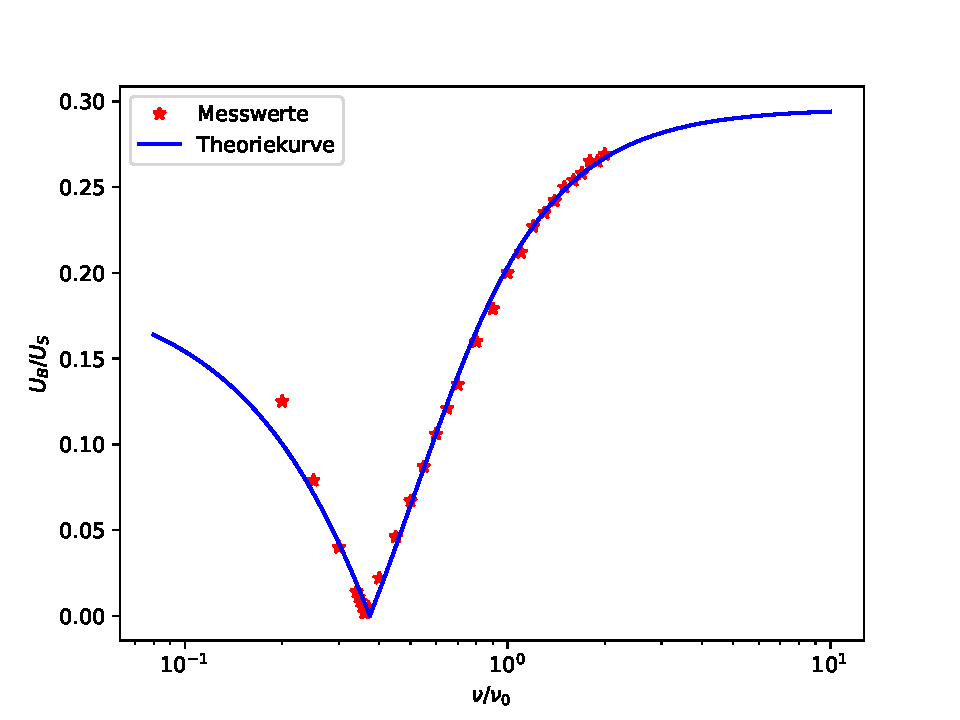
\includegraphics[scale=0.7]{plotFrequenz2.pdf}
  \caption{Gemessene Werte bei der Wien-Robinson-Brücke}
  \label{fig:1}
\end{figure}
%\newpage
\subsection{Klirrfaktor}
Der Klirrfaktor lässt sich durch
\begin{equation}
  k \coloneq \frac{\sqrt []{U_2^2+U_3^2+\dotsc}}{U_1}
\end{equation}
berechnen. Hierbei wird ausschließtlich die zweite Oberwelle betrachtet. Die Werte
für $\su{U_2}$ und $\su{U_1}$ werden zur Berechnung noch bestimmt,
wobei $\su{U_1}$ die 2.08 V von $\su{U\ua{B}}$ bei $\su{\nu_0}$ sind. Mit \ref{eqn:WiRo}
%Formel aus der Theorie an der Stelle
und $\su{\Omega}$ = 2 folgt dann:
\begin{align*}
  \su{U_2} &= \frac{U\ua{B}}{\sqrt{\frac{(2^2 -1)^2}{9 [(1-2^2)^2 + 9 \cdot 2^2]}}} \\
           &= 0.0147 \, \su{V}.
\end{align*}


Der Klirrfaktor ergibt sich dann aus dem Quotienten von $\su{U_2}$ und
$\su{U_1}$:
\begin{equation*}
  \su{k} = \frac{\su{U_2}}{\su{U_1}} = 7.067 \cdot 10^{-3}.
\end{equation*}

\section{Diskussion}
Bei der Untersuchung verschiedener Brückenschaltungen war besonders das Finden des Minimuns
fehleranfällig. Hierbei spielte sowohl der regelbare Widerstand, als auch das Oszilloskop
eine entscheidene Rolle. Mithilfe des regelbaren Widerstands war das Minimum zum Teil gar
nicht auffindbar, da dieser schon bis zum Anschlag aufgedreht war. Außerdem konnte wegen
Schwankungen auf dem Oszilloskop das Minimum nicht genau eingestellt werden.
\newline
Zusammen führte dies zu einer großen Minimunsspannweite und könnte Abweichungen erklären.

Die gemessen Kapazitäten haben größere Fehler als die Ohmschen Widerstände. Diese Messung
zeigte bereits während der Durchführung des Versuchs eine größere Empfindlichkeit gegenüber
Stößen. Bei der Induktivitätsmessung zeigen sich größere Unterschiede zwischen den beiden
Messmethoden. Besonders die verwendete Spule zeigten dabei eine große Abweichung. Die Induktivität
ist bei der Wien-Robinson-Brücke viel größer. Durch das dreimalige Bestimmen der Induktiät
mithile der Wien-Robinson-Brücke und des relativ geringen Fehlers scheint diese Messung zuverlässiger zu sein.

Des Weitern lassen sich Abweichungen im Graphen der Messwerte der Wien-Robinson-Brücke im
Vergleich mit der Theoeriekurve feststellen. Für die Anpassung an die Messwerte mussten dabei
die Paramter der Theoriefunktion verringert werden. Eine mögliche Ursache dafür könnte sein,
dass etwaige Verluste der Bauteile bei niedrigen und hohen Frequenzen und Spannungsschwankungen auftreten.
